\paragraph{Law of cosine}
\begin{center}	
	\includesvg[eps,svgpath = lect2/,width=0.2\linewidth]{pic1}
\end{center}
$$\vec{C} = \vec{A} - \vec{B}=\vec{A} + (-\vec{B})$$
$$(\vec{A}-\vec{B}) \cdot (\vec{A}-\vec{B}) = \vec{C} \cdot \vec{C}$$
$$A^2+B^2-2AB\cos \alpha = C^2$$

\paragraph{Power} Rate of doing work

$$W = LF\cos \alpha = \vec{L} \cdot \vec{F}$$

In a short time $dt$ a body passed a short distance $dL$.
So $dW=d\vec{L} \cdot {F}$

Then $power = \frac{dW}{dt} = \frac{d\vec{L}}{dt} \cdot \vec{F} = \vec{v} \cdot \vec{F}$


\subparagraph{Units} Units are:


Force  - $N$

Energy - $J$

Power -  $W$

\subsection{Cartesian coordinate system}

\begin{center}
	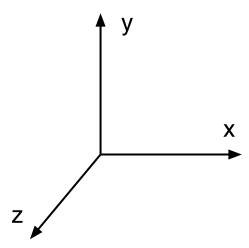
\includegraphics[width=0.2\linewidth]{./lect2/pic2.png}
\end{center}

\begin{align*}
\vec{A} \times \vec{B}  &\mathrlap{= (A_x\hat{x} + A_y\hat{y} + A_z\hat{z})\times (B_x\hat{x} + B_y\hat{y} + B_z\hat{z}) =}\\
&= A_xB_x(\hat{x} \times \hat{x}) &+ A_xB_y(\hat{x} \times \hat{y}) &+ A_xB_z(\hat{x} \times\hat{z})+\\ 
&&+A_yB_x(\hat{y} \times \hat{x}) &+ A_yB_y(\hat{y} \times \hat{y}) + A_yB_z(\hat{y} \times \hat{z}) +\\
&&&+ A_zB_x(\hat{z} \times \hat{x}) + A_zB_y(\hat{z} \times \hat{y}) + A_zB_z(\hat{z} \times \hat{z}) =\\
&&& = (A_yB_z -  A_zB_y)\hat{x}  + (A_zB_x + A_xB_z)\hat{y} + (A_xB_y - A_yB_x)\hat{z}
\end{align*}



\subsection{Usages}

\paragraph{Area of parallelogram}
\begin{center}	
	\includesvg[eps,svgpath = lect2/,width=0.5\linewidth]{pic3}
\end{center}
$h$ is an altitude.

$S  = ah = ab \sin \theta = \mid \vec{a} \times \vec{b} \mid\\
\vec{S} = \vec{a} \times \vec{b}$

If there is a curved surface area vector is perpendicular to surface in every point.
\paragraph{Parallelepiped volume}
\begin{center}	
	\includesvg[eps,svgpath = lect2/,width=0.7\linewidth]{pic4}
\end{center}
Two equal parallel parallelogram defined with $\vec{b}, \vec{c}$ and $\vec{a}$ is a vector between them.

$\vec{S} = \vec{b} \times \vec{c}\\
h = \mid \vec{a} \mid \cos \alpha\\
V = S \cdot h = \mid \vec{S} \cdot \vec{a} \mid = \mid (\vec{b} \times \vec{c}) \cdot \vec{a} \mid$

Same order (a,b,c), no matter which are used for cross product gives same result: $(\vec{a}\times \vec{b}) \cdot \vec{c} = \vec {b} \cdot (\vec{c} \times \vec{a})$. However different order (b,a,c), e.g. $(\vec{a}\times \vec{c}) \cdot \vec{b}$ will give opposite sign.

\paragraph{Law of sines}

$\vec{C} = \vec{A} + \vec{B}\\
\vec{A} \times \vec{C} = \vec{A} \times \vec{A}+ \vec{A} \times \vec{B} = \vec{A} \times \vec{B}\\
\mid \vec{A} \times \vec{C} \mid = \mid \vec{A} \times \vec{B}\mid\\
AC\sin \beta = AB\sin \gamma\\
\frac{C}{\sin \gamma} = \frac{B}{\sin \beta}$

